%Este trabalho está licenciado sob a Licença Atribuição-CompartilhaIgual 4.0 Internacional Creative Commons. Para visualizar uma cópia desta licença, visite http://creativecommons.org/licenses/by-sa/4.0/deed.pt_BR ou mande uma carta para Creative Commons, PO Box 1866, Mountain View, CA 94042, USA.

\chapter{Aplicações da derivada}\label{cap_apderiv}
\thispagestyle{fancy}

\ifispython
\begin{obs}
  Nos códigos \verb+Python+ apresentados neste capítulo, assumimos o seguinte preâmbulo:
\begin{verbatim}
from sympy import *
var('x',real=True)
\end{verbatim}
\end{obs}
\fi

\section{Extremos de funções}\label{cap_apderiv_sec_extfun}

Seja $f$ uma função com domínio $D$. Dizemos que $f$ tem valor \emph{máximo absoluto} no ponto $x=a$ quando
\begin{equation}
  f(x) < f(a),
\end{equation}
para todo $x\in D$. Analogamente, dizemos que $f$ tem valor \emph{mínimo absoluto} no ponto $x=b$ quando
\begin{equation}
  f(x) > f(b),
\end{equation}
para todo $x\in D$.

\begin{ex}\label{ex:vmaxminabs}
  A função $f(x) = x^2$ tem valor mínimo absoluto no ponto $x=0$ e não assume valor máximo absoluto. A função $g(x) = -x^2$ tem valor máximo absoluto no ponto $x=0$ e não assume valor mínimo absoluto. A função $h(x)=x^3$ não assume valores mínimo e máximo absolutos. Veja a Figura \ref{fig:ex_vmaxminabs}.

  \begin{figure}[H]
    \centering
    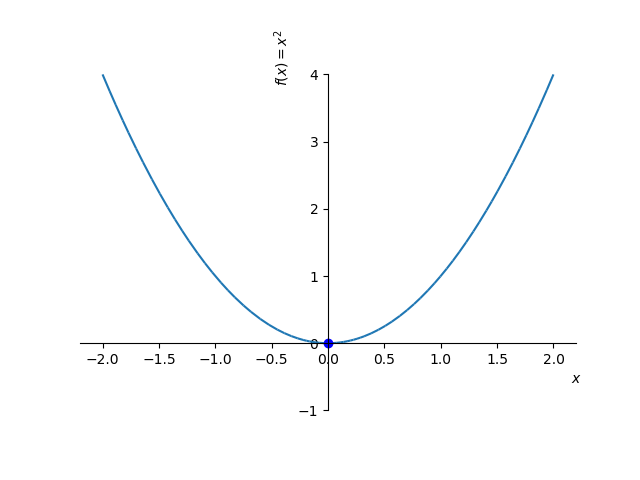
\includegraphics[width=0.3\textwidth]{./cap_apderiv/dados/fig_ex_vmaxminabs/fig_f}~
    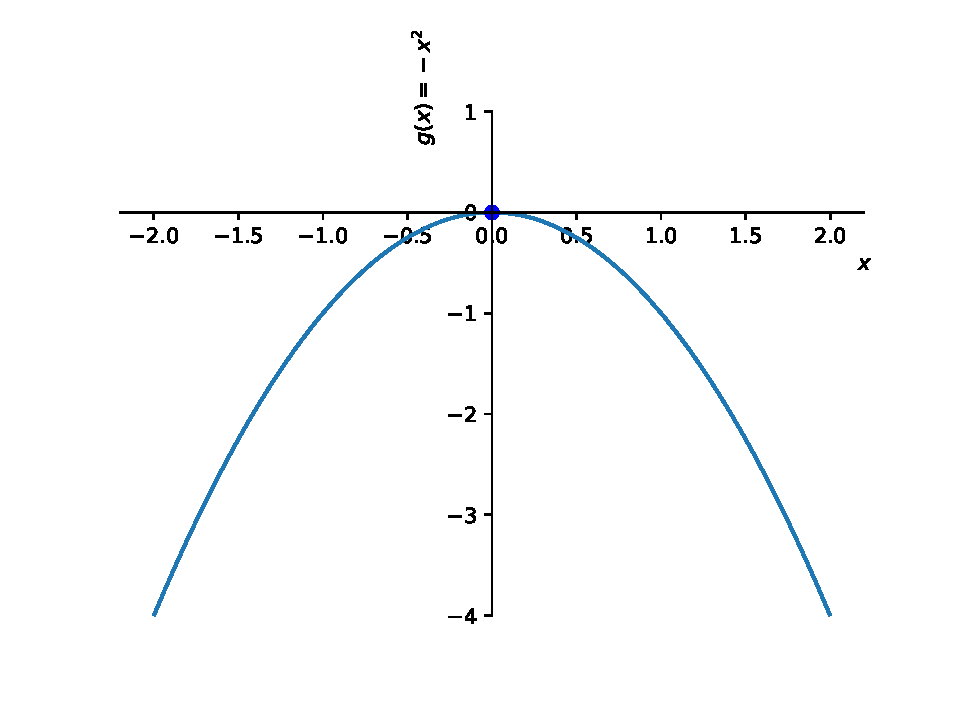
\includegraphics[width=0.3\textwidth]{./cap_apderiv/dados/fig_ex_vmaxminabs/fig_g}~
    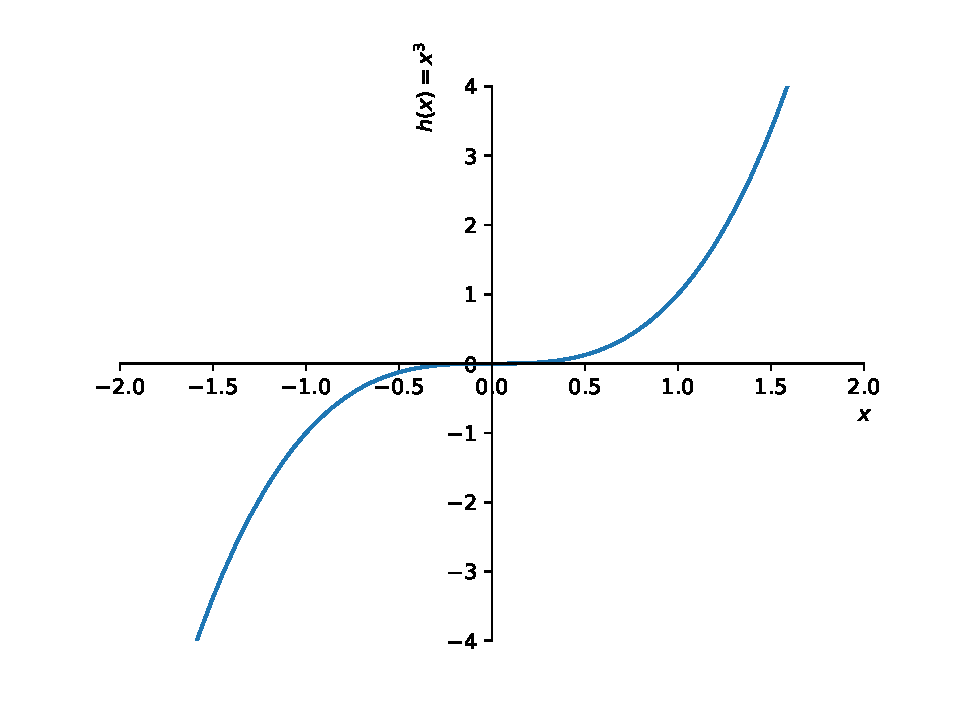
\includegraphics[width=0.3\textwidth]{./cap_apderiv/dados/fig_ex_vmaxminabs/fig_h}
    \caption{Esboço das funções discutidas no Exemplo \ref{ex:vmaxminabs}.}
    \label{fig:ex_vmaxminabs}
  \end{figure}
\end{ex}

\begin{teo}\normalfont{(Teorema do valor extremo)}
  Se $f$ é uma função contínua em um intervalo fechado $[a, b]$, então $f$ assume tanto um valor máximo como um valor mínimo absoluto em $[a, b]$.
\end{teo}

\begin{ex}\label{ex:fcont}
  Vejamos os seguintes casos:
  \begin{enumerate}[a)]
  \item  A função $f(x) = (x-1)^2+1$ é contínua no intervalo fechado $[0,\frac{3}{2}]$. Assume valor mínimo absoluto de $1$ no ponto $x=1$. Ainda, assume valor máximo absoluto igual a $2$ no ponto $x=0$. Veja Figura \ref{fig:ex_fcont_f}.
  \begin{figure}[H]
    \centering
    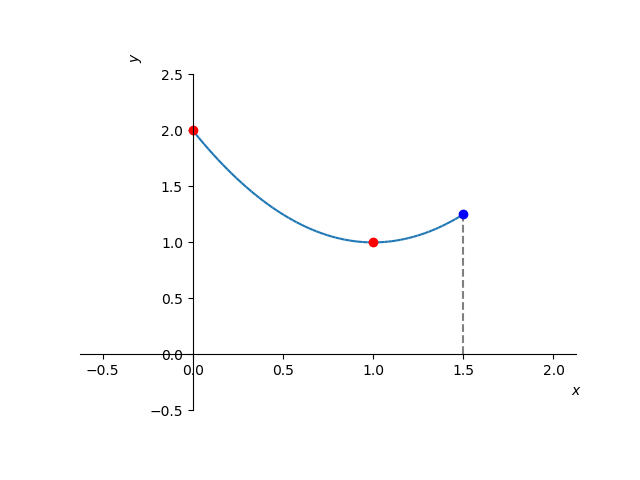
\includegraphics[width=0.5\textwidth]{./cap_apderiv/dados/fig_ex_fcont/fig_f}
    \caption{Esboço do gráfico de $f(x) = (x-1)^2+1$ no intervalo $[0,\frac{3}{2}]$. Veja o Exemplo \ref{ex:fcont} a).}
    \label{fig:ex_fcont_f}
  \end{figure}
\item A função $g(x) = \ln x$ é contínua no intervalo $(0, e]$. Neste intervalo, assume valor máximo absoluto no ponto $x=e$, mas não assume valor mínimo absoluto. Veja Figura \ref{fig_ex_fcont_g}.
  \begin{figure}[H]
    \centering
    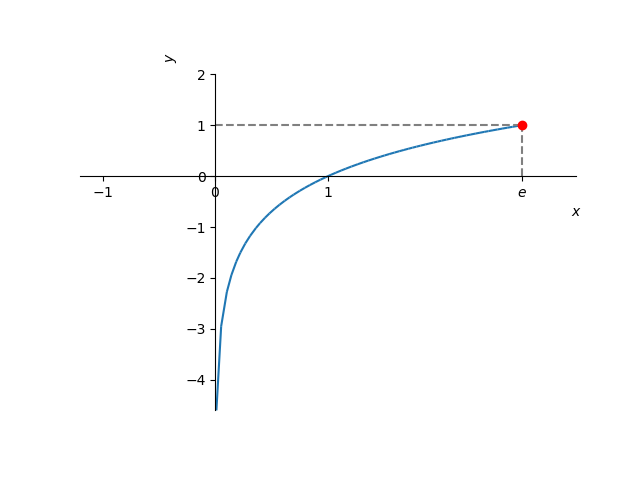
\includegraphics[width=0.5\textwidth]{./cap_apderiv/dados/fig_ex_fcont/fig_g}
    \caption{Esboço do gráfico de $g(x) = \ln x$ no intervalo $(0,e]$. Veja o Exemplo \ref{ex:fcont} b).}
    \label{fig:ex_fcont_g}
  \end{figure}
  
\item A função
  \begin{equation}
    g(x) = \left\{
      \begin{array}{ll}
        x &, 0<x<1,\\
        0 &, x=1,
      \end{array}
\right.
\end{equation}
definida no intervalo $[0,1]$ é descontínua no ponto $x=1$. Neste intervalo, assume valor mínimo absoluto no ponto $x=0$, mas não assume valor máximo absoluto.
  \end{enumerate}
\end{ex}

\emconstrucao